% !TeX spellcheck = es_ES
\documentclass[a4paper,12pt]{article}
\usepackage[utf8]{inputenc}
\usepackage{graphicx}
\usepackage{float}
\usepackage{listings}
\usepackage{color}
\usepackage[spanish]{babel}
\usepackage[nottoc,notlot,notlof]{tocbibind} % Hace que se agregen las referencias al indice
 
\definecolor{codegreen}{rgb}{0,0.6,0}
\definecolor{codegray}{rgb}{0.5,0.5,0.5}
\definecolor{codepurple}{rgb}{0.58,0,0.82}
\definecolor{backcolour}{rgb}{0.95,0.95,0.92}
 
\lstdefinestyle{mystyle}{
    backgroundcolor=\color{backcolour},   
    commentstyle=\color{codegreen},
    keywordstyle=\color{magenta},
    numberstyle=\tiny\color{codegray},
    stringstyle=\color{codepurple},
    basicstyle=\footnotesize,
    breakatwhitespace=false,         
    breaklines=true,                 
    captionpos=b,                    
    keepspaces=true,                 
    numbers=left,                    
    numbersep=5pt,                  
    showspaces=false,                
    showstringspaces=false,
    showtabs=false,                  
    tabsize=2
}
 
\lstset{style=mystyle}

%opening
\title{Maquina de Turing que duplica la cantidad de unos}
\author{Barrera Pérez Carlos Tonatihu \\ Profesor: Genaro Juárez Martínez \\ Computing Selected Topics \\ Grupo: 3CM8 }

\begin{document}

\maketitle
\newpage
\tableofcontents
\newpage
\section{Introducción}
La elaboración de este programa consistió en elaborar un maquina de Turing capaz de duplicar la cantidad de unos en una cadena de unos, es decir, si la cadena que se ingresa es $ 11 $ entonces la cadena de salida sera $ 1111 $.

Es por esto que la maquina sólo aceptara unos en la entrada mientras que los símbolos de la cinta incluirán a la X y la Y. De esta forma la maquina de Turing para este problema se define como:

\[M=(\lbrace q_{0}, q_{1}, q_{2}, q_{3}\rbrace, \lbrace 1 \rbrace, \lbrace 1, X, Y, B \rbrace, \delta, q_{0}, B, \lbrace q_{4} \rbrace)\]

donde $ \delta $ se especifica en la siguiente tabla:
\begin{center}
\begin{tabular}{|c|c|c|c|c|}
\hline
& \multicolumn{4}{|c|}{Símbolo} \\ \hline
Estado & 1 & X & Y & B\\ \hline
0 & (1, X, R) & - & (3, 1, R) & -\\ \hline
1 & (1, 1, R) & - & (1, Y, R) & (1, Y, L)\\ \hline
2 & (2, 1, L) & (0, 1, R) & (2, Y, L) & -\\ \hline
3 & - & - & (3, 1, R) & - \\ \hline
\end{tabular}
\end{center}

EL funcionamiento de esta maquina se puede entender mejor con el diagrama de la figura \ref{fig:diagrama}

\begin{figure}[H]
\begin{center}
 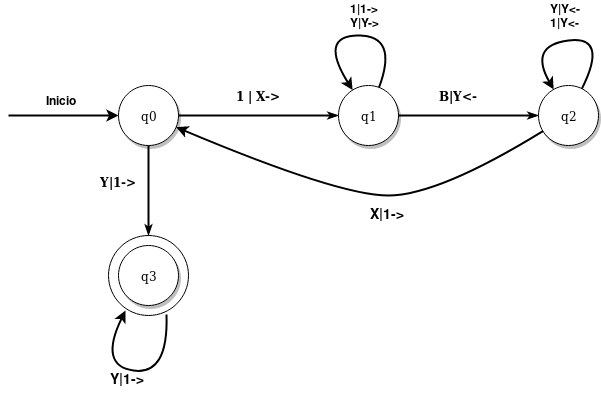
\includegraphics[width=12cm, height=7cm]{Turing-unos.png}
 \caption{Representación gráfica de las transiciones de la maquina de Turing}
 \label{fig:diagrama}
\end{center}
\end{figure}

El funcionamiento del programa empieza cuando se inserta una cadena de unos y la maquina empezara a trabajar, además de generar una cadena final se muestra una animación del como se están realizando las transiciones en la cinta de la maquina, por otro lado se imprime en consola el historial de movimientos que se hacen, este historial también se guarda en un archivo de texto.

\section{Desarrollo}
El código de este programa fue realizado en Python 3.7 y se utilizo la biblioteca tkinter para la parte gráfica.

Archivo: turing.py
Esta clase es la que modela la maquina de Turing, los parámetros importantes son: el estado inicial, los estados finales, la cadena de entrada y la función de transición.
\begin{lstlisting}[language=Python]
class MaquinaTuring:
    """MaquinaTuring"""
    def __init__(self, estado_inicial, estados_finales, cadena, transiciones):
        self.transiciones = transiciones
        self.inicial = estado_inicial
        self.finales = estados_finales
        self.cinta = list(cadena)
        self.estado_actual = self.inicial
        self.apuntador = 0
        self.blanco = "B"
        self.direccion = None

    def consumir(self):
        """Toma un simbolo de la cinta y lo evalua en la funcion de
        transicion"""
        if len(self.cinta) - 1 < self.apuntador:
            caracter = 'B'
        else:
            caracter = self.cinta[self.apuntador]
        tupla = (self.estado_actual, caracter)
        if tupla in self.transiciones:
            siguiente = self.transiciones[tupla]
            if len(self.cinta) - 1 < self.apuntador:
                self.cinta.append(self.blanco)
            if self.apuntador < 0:
                self.cinta.insert(0, self.blanco)
            self.cinta[self.apuntador] = siguiente[1]
            if siguiente[2] == "R":
                self.apuntador += 1
            else:
                self.apuntador -= 1

            self.estado_actual = siguiente[0]
            self.direccion = siguiente[2]
            return True
        else:
            return False

    def es_final(self):
        """Metodo para comprobar si nos encontramos en un estado final"""
        if self.estado_actual in self.finales:
            if len(self.cinta) - 1 < self.apuntador or self.apuntador < 0:
                return True
        return False
\end{lstlisting}

Archivo: diagrama.py
Este archivo implementa la clase MaquinaTuring.py y se declaran los parámetros que se pasaran a este archivo así como la captura de la cadena y la escritura del registro de transiciones en consola y en archivo de texto, sin olvidar la animación de dichas transiciones.
\begin{lstlisting}[language=Python]
import tkinter as tk
import time
from tkinter import font as tkfont
from turing import MaquinaTuring

# Tabla de transiciones que modela el automata
transiciones = {
            ("q0", "1"): ("q1", "X", "R"),
            ("q0", "Y"): ("q3", "1", "R"),
            ("q1", "1"): ("q1", "1", "R"),
            ("q1", "Y"): ("q1", "Y", "R"),
            ("q1", "B"): ("q2", "Y", "L"),
            ("q2", "1"): ("q2", "1", "L"),
            ("q2", "X"): ("q0", "1", "R"),
            ("q2", "Y"): ("q2", "Y", "L"),
            ("q3", "Y"): ("q3", "1", "R"),
            }

entrada = input("Ingrese la cadena de unos: ")
maquina = MaquinaTuring("q0", "q3", entrada, transiciones)

# Configuracion de la ventana
gui = tk.Tk()
gui.geometry("600x400+100+100")
gui.title("Maquina de Turing")
c = tk.Canvas(gui, width=600, height=400)
c.pack()
bold_font = tkfont.Font(family="Arial", size=24)

# Principales componentes que se animan
control = c.create_rectangle(150, 100, 200, 150, fill="lightblue")
flecha = c.create_line(175, 150, 175, 175, arrow=tk.LAST, width=3)
texto = c.create_text(165, 200, text=''.join(maquina.cinta), font=bold_font,
                      anchor=tk.W)
estado = c.create_text(160, 125, text=maquina.estado_actual, font=bold_font,
                       anchor=tk.W)

archivo = open("salida.txt", "w+")
# Mientras no llegues a un estado final continua
while not maquina.es_final():
    print('Cadena: {}'.format(''.join(maquina.cinta)))
    print('Estado actual: {}, apuntador: {}'.format(maquina.estado_actual,
          maquina.apuntador+1))

    archivo.write('Cadena: {}\n'.format(''.join(maquina.cinta)))
    archivo.write('Estado actual: {}, apuntador: {}\n'
                  .format(maquina.estado_actual, maquina.apuntador+1))
    if not maquina.consumir():
        print('*' * 20)
        archivo.write('*' * 20)
        archivo.write('\n')
        break
    print('Siguiente estado: {}'.format(maquina.estado_actual))
    print('*'*20)

    archivo.write('Siguiente estado: {}\n'.format(maquina.estado_actual))
    archivo.write('*' * 20)
    archivo.write('\n')

    gui.update()
    time.sleep(1)
    c.itemconfigure(texto, text=''.join(maquina.cinta), anchor=tk.W)
    c.itemconfigure(estado, text=maquina.estado_actual)
    if maquina.direccion == 'R':
        c.move(control, 19, 0)
        c.move(flecha, 19, 0)
        c.move(estado, 19, 0)
    else:
        c.move(control, -19, 0)
        c.move(estado, -19, 0)
        c.move(flecha, -19, 0)

print('Cadena final: {}'.format(''.join(maquina.cinta)))
archivo.write('Cadena final: {}\n'.format(''.join(maquina.cinta)))
archivo.close()
gui.mainloop()
\end{lstlisting}

\section{Pruebas}
El siguiente ejemplo es la cadena con un solo uno.

\begin{figure}[H]
\begin{center}
 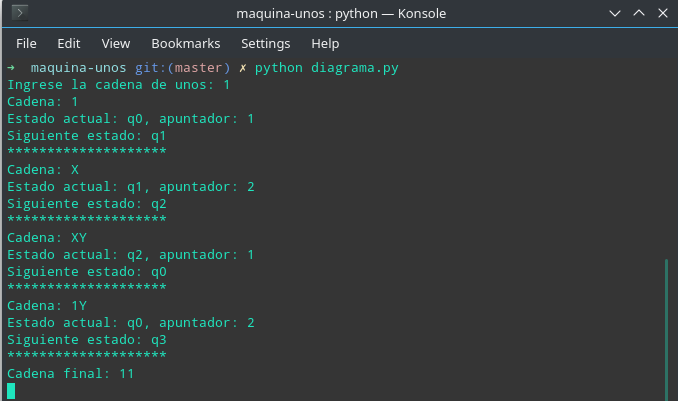
\includegraphics[width=13cm, height=8cm]{uno_consola.png}
 \caption{Salida en consola}
 \label{fig:uno_consola}
\end{center}
\end{figure}

\begin{figure}[H]
\begin{center}
 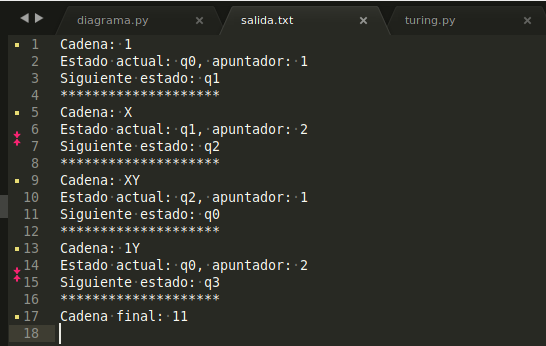
\includegraphics[width=13cm, height=8cm]{uno_historial.png}
 \caption{Registro de transiciones}
 \label{fig:uno_historial}
\end{center}
\end{figure}

\begin{figure}[H]
\begin{center}
 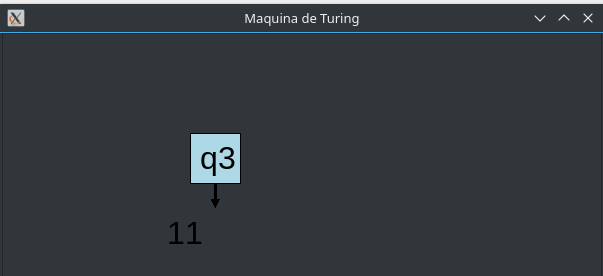
\includegraphics[width=13cm, height=6cm]{uno_grafica.png}
 \caption{Representación gráfica de las transiciones de la maquina de Turing}
 \label{fig:uno_grafica}
\end{center}
\end{figure}

En este ejemplo se inserta una cadena con dos unos.
\begin{figure}[H]
\begin{center}
 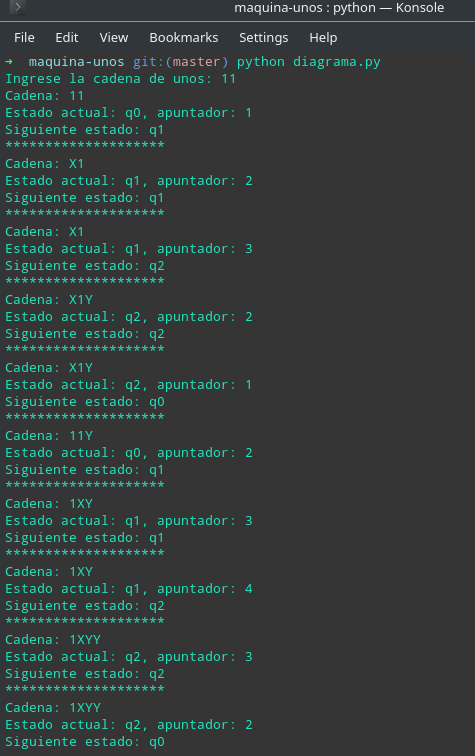
\includegraphics[width=13cm, height=20cm]{dos_consola.png}
 \caption{Salida en consola parte uno}
 \label{fig:dos_consola}
\end{center}
\end{figure}

\begin{figure}[H]
\begin{center}
 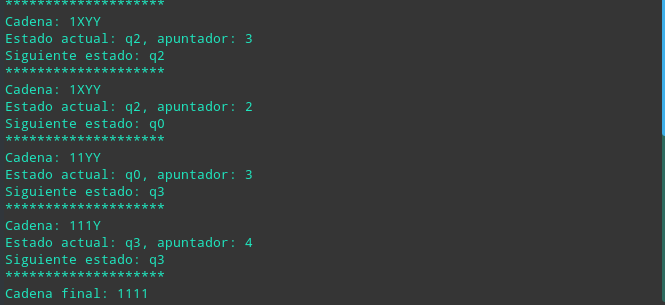
\includegraphics[width=13cm, height=7cm]{dos_console.png}
 \caption{Salida en consola parte dos}
 \label{fig:dos_console}
\end{center}
\end{figure}

\begin{figure}[H]
\begin{center}
 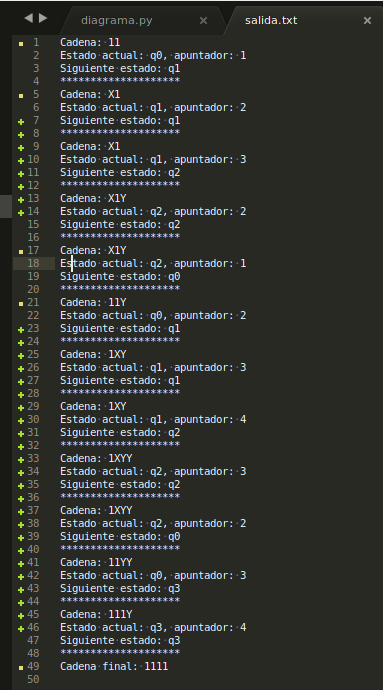
\includegraphics[width=13cm, height=20cm]{dos_historial.png}
 \caption{Registro de transiciones}
 \label{fig:dos_historial}
\end{center}
\end{figure}

\begin{figure}[H]
\begin{center}
 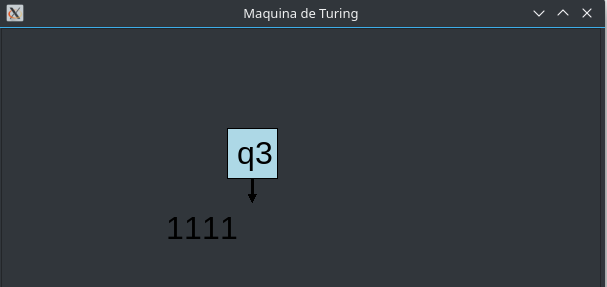
\includegraphics[width=13cm, height=6cm]{dos_grafica.png}
 \caption{Representación gráfica de las transiciones de la maquina de Turing}
 \label{fig:dos_grafica}
\end{center}
\end{figure}

\nocite{LIBRO}

\bibliographystyle{ieeetr}
\bibliography{reporte}

\end{document}
